\documentclass{beamer}
\usepackage[utf8]{inputenc}
\usepackage{hyperref}

\usepackage{tikz}

\usepackage{latexsym,xcolor,multicol,booktabs,calligra}
\usepackage{amsmath,amssymb,BOONDOX-cal,bm}	
\usepackage{graphicx,pstricks,stackengine} 
\usepackage{libertinus}
\usepackage{amssymb}
\usepackage{pgfplots}
\usepackage{tikz}
\usepackage{xcolor}
\usetikzlibrary{positioning}

\usepackage{etoolbox}
\makeatletter
\newcommand{\noframenumbering}{%
  \beamer@noframenumberingtrue%
}
\makeatother

\usepackage[T1]{fontenc}

\title{Macroeconometrics\\
1 Introduction to Time Series}
\author{Camille Souffron\\
Ecole Normale Supérieure \& Paris School of Economics\\
\textcolor{blue}{\href{mailto:camille.souffron@ens.psl.eu}{camille.souffron@ens.psl.eu}}}
\institute{\normalsize M2 EPOG JM}
\date{Fall 2026}

\usetheme{Singapore}

\def\cmd#1{\texttt{\color{red}\footnotesize $\backslash$#1}}
\def\env#1{\texttt{\color{RoyalBlue}\footnotesize #1}}

\newtheorem{thm}{Theorem}[theorem]
\setbeamertemplate{footline}[frame number]

\begin{document}

\begin{frame} % <-- no [plain] here!
    \titlepage % This keeps the theme style
    \begin{center}
        
\includegraphics[width=0.5\textwidth]{logos.png}
    \end{center}
\end{frame}



\addtocounter{framenumber}{-1}







\section{Introduction}
% Roadmap
\begin{frame}{Course Roadmap}
\small
\begin{enumerate}
  \item \textbf{Introduction to Time Series Analysis}  

  \item \textbf{AR, MA, ARMA Processes and Filtering Methods}  

  \item \textbf{VAR Models and Local Projections}  

  \item \textbf{Structural VARs, Identification and Policy Impact}  
  Short- and long-run restrictions, sign restrictions, proxy-SVARs, Instruments.

  \item \textbf{Nonlinear Models}  
  Threshold (TAR), Smooth Transition (STAR), and Markov-Switching Regimes.

  \item \textbf{Dynamic Factor and State-Space Models}  

  \item \textbf{Calibration \& Estimation of Structural Models I}  
  Empirical SFC \& IO.

  \item \textbf{Calibration \& Estimation of Structural Models II}  
  GMM, SMM, and Backtesting.

  \item \textbf{Calibration \& Estimation of Structural Models III}  
  Agent-Based Models (ABM).

  \item \textbf{Bibliometrics, Meta-Analysis \& Spectral Methods}  
  Measuring consensus, publication bias, and frequency domain.
\end{enumerate}
\end{frame}


% ——————————————————————————————————————————
% Section 1: Introduction to Time Series
% ——————————————————————————————————————————




\begin{frame}{Introduction}
    Specific textbooks in time series (but do not cover all the course AND do not show how to use time series to estimate structural models):
    
\begin{itemize}
\item Hamilton J.D. (1994), Time Series Analysis, Princeton Univ. Press.
\item Lütkepohl H. (2005), New Introduction to Multiple Time Series Analysis, Springer Verlag.
\item  Brockwell P.J., Davis A. (2002) Introduction to Time Series and Forecasting (2nd ed.) Springer.
\item  Brockwell P.J., Davis A. (2006) Time Series: Theory and Methods (2nd ed.) Springer.
\end{itemize}
\end{frame}


\begin{frame}{Introduction}
    \begin{itemize}
        \item Programming language: $R$
        \item IDE: $R$ Studio.
        \item Please install both of them for the next class.
\end{itemize}
\end{frame}


\begin{frame}{Introduction}
\begin{itemize}
    \item A \textbf{univariate time series} is a set of observations $x_t$ of a real variable $x$, observed at time $t$, $t = 1, \ldots, T$.
    \vspace{0.2cm}
    \item \textbf{Examples in macroeconomics:} quarterly GDP, annual GDP per capita, quarterly aggregate consumption, monthly industrial production, monthly result of a business survey, etc.
    \vspace{0.2cm}
    \item \textbf{Other examples:} annual number of road traffic accidents, daily number of COVID cases in a country, monthly number of international airline passengers, weekly sales of a shop, monthly number of real estate transactions, etc.
    \vspace{0.2cm}
    \item \textbf{Two types of data:}
    \begin{itemize}
        \item low frequency: annual, quarterly, monthly, weekly data
        \item high frequency: daily, intraday data
    \end{itemize}
    \vspace{0.2cm}
    \item \textbf{Two approaches:}
    \begin{itemize}
        \item low frequency data: \textcolor{blue}{discrete time} ($t \in \mathbb{N}$ or $t \in \mathbb{Z}$)
        \item high frequency data: \textcolor{blue}{continuous time} ($t \in \mathbb{R}$)
    \end{itemize}
\end{itemize}
\end{frame}

\begin{frame}{Introduction}
    \begin{itemize}
  \item \textbf{tradeoff}: number of observations vs historical span
  \begin{itemize}
    \item \textbf{Macroeconomic variables}: study of \textit{growth trends} $\rightarrow$ techniques: \textbf{unit roots}, \textbf{cointegration}.
    \item \textbf{Financial variables}: study of \textit{volatility} $\rightarrow$ methods: \textbf{AutoRegressive Conditional Heteroskedasticity (ARCH)} and extensions.
  \end{itemize}
\end{itemize}
\end{frame}



\begin{frame}{Introduction}
\begin{itemize}
    \item This course: \textcolor{blue}{discrete time only.}
    \vspace{0.2cm}
    \item To estimate models, it is necessary to have enough data: the models presented here will mainly be applied to quarterly or monthly data.
    \vspace{0.2cm}
    \item $x_t$ is seen as the \textbf{realization of a random variable} $X_t$, which is defined for any $t \in \mathbb{Z}$.
    \vspace{0.2cm}
    \item $(X_t)_{t \in \mathbb{Z}}$ is called a \textbf{stochastic process}.
    \vspace{0.2cm}
    \item $\{x_t, t = 1, \ldots, T\}$ is a \textbf{trajectory} of the process $(X_t)_{t \in \mathbb{Z}}$.
    \vspace{0.3cm}
    \item \textbf{Important remarks:}
    \begin{itemize}
        \item Most often the realization and the random variable are denoted the same way (indifferently $x_t$ or $X_t$).
        \item “Time series” and “stochastic process” are often used interchangeably.
        \item Time data $\neq$ individual data: they are \textbf{ordered in time!} \\
        What happens today is linked to what happened before.
    \end{itemize}
\end{itemize}
\end{frame}

% ——————————————————————————————————————————
% Additive model
% ——————————————————————————————————————————
\begin{frame}{The additive model}
\small
Simple model of time series, involving:
\begin{itemize}
  \item \textbf{Deterministic components:} trend and seasonality.
  \item \textbf{Plus a random or stochastic component} which shows no informative pattern.
\end{itemize}

\medskip
Let $X_t$ be a time series described by the following model:
\[
X_t = m_t + s_t + \varepsilon_t, \quad t = 1, \ldots, T
\]
where:
\begin{itemize}
  \item $m_t$: trend component (or mean level) at time $t$;
  \item $s_t$: seasonal component at time $t$, of period $d$;
  \item $\varepsilon_t$: random noise sequence at time $t$.
\end{itemize}
\end{frame}


\begin{frame}
\begin{figure}
    \centering
    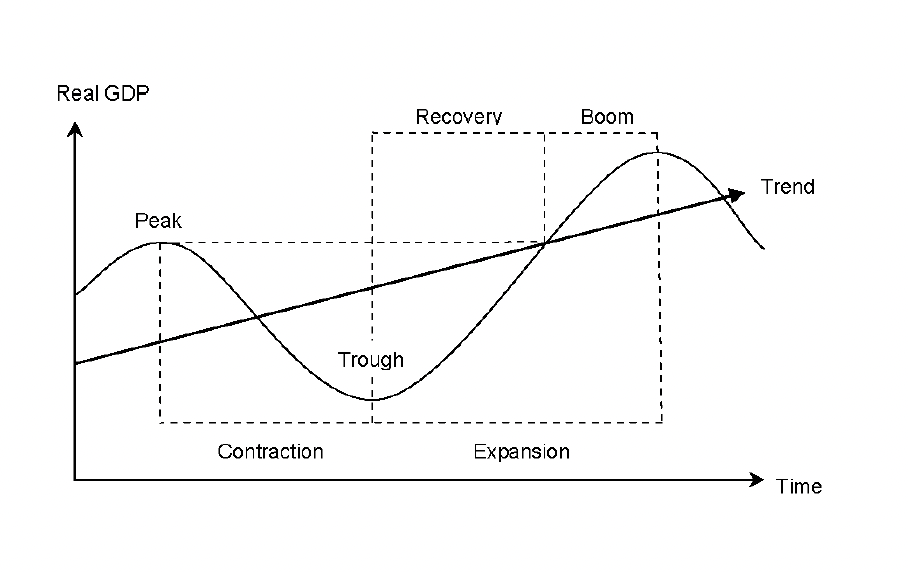
\includegraphics[width=1\linewidth]{Capture d’écran 2025-10-14 à 22.57.26.png}
    \caption{Example: business cycle}
\end{figure}
\end{frame}

% ——————————————————————————————————————————
% Multiplicative model
% ——————————————————————————————————————————
\begin{frame}{The multiplicative model}
\small
\[
X_t = M_t \times S_t \times \varepsilon_t, \quad t = 1, \ldots, T
\]

\pause
\textbf{Study of } $\log X_t$:
\[
\log X_t = \log M_t + \log S_t + \log \varepsilon_t, \quad t = 1, \ldots, T
\]

\[
\Rightarrow
\begin{cases}
m_t = \log M_t,\\
s_t = \log S_t,\\
\varepsilon_t = \log \varepsilon_t.
\end{cases}
\]
\end{frame}




\begin{frame}{The classical decomposition of a time series}
\begin{figure}
        \centering
        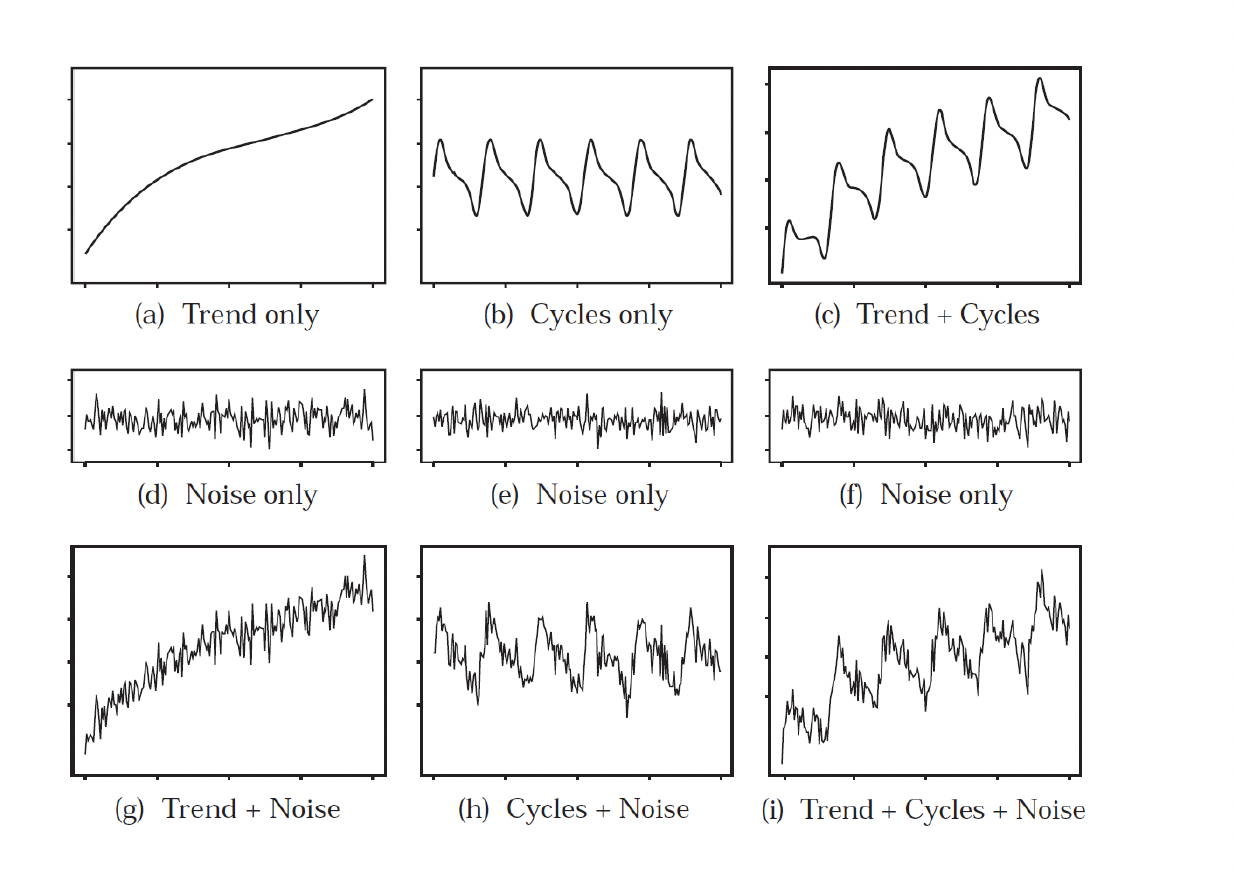
\includegraphics[width=\linewidth]{Capture d’écran 2025-10-14 à 22.59.28.png}
    \end{figure}
        
\end{frame}

% ——————————————————————————————————————————
% A time series is a stochastic process
% ——————————————————————————————————————————

\begin{frame}{A time series is a stochastic process.}
\small
\begin{itemize}
    \[
    (X_t)_{t=1,\ldots,T}, \quad \text{referred to as the \textbf{stochastic process}.}
    \]
    \vspace{0.2cm}
    \item \textbf{Idea:} if we could rerun history $M$ times, we would obtain $M$ different sample paths:
    \[
    \Rightarrow \text{$M$ realized sample paths = $M$ observed time series.}
    \]
\end{itemize}

\vspace{0.4cm}
\centering
\begin{tabular}{cccccc}
\textbf{Realization 1} & $x_1^{(1)}$ & $\cdots$ & $x_t^{(1)}$ & $\cdots$ & $x_T^{(1)}$ \\
$\vdots$ & $\vdots$ & & $\vdots$ & & $\vdots$ \\
\textbf{Realization $m$} & $x_1^{(m)}$ & $\cdots$ & $x_t^{(m)}$ & $\cdots$ & $x_T^{(m)}$ \\
$\vdots$ & $\vdots$ & & $\vdots$ & & $\vdots$ \\
\textbf{Realization $M$} & $x_1^{(M)}$ & $\cdots$ & $x_t^{(M)}$ & $\cdots$ & $x_T^{(M)}$ \\
\end{tabular}
\end{frame}

% ——————————————————————————————————————————
% Objective + Modelling logic
% ——————————————————————————————————————————

\begin{frame}{Introduction}
\begin{itemize}
  \item Our (\textit{very ambitious}) objective: \textbf{Find the best process $(X_t)$ that generated $x_t$}.
  \item (\textit{For mathy people, go study Lebesgue measure: core of probability and of stochastic process (and of integration).})
\end{itemize}
\end{frame}

\begin{frame}{Introduction}
\textbf{From modelling to forecasting}
\begin{itemize}
  \item If the process has been (i) specified, (ii) estimated and (iii) validated, it can be used for \textbf{forecasting} and for \textbf{assessing the impact of shocks}.
  \item We note $\hat X_T(h)$ the \textbf{predictor} of $X_{T+h}$.
  \item As an estimator, this predictor is a \textbf{random variable}, i.e. a measurable function of random variables.
  \item Thus, $\hat X_T(h)$ has its \textbf{own distribution}, which we must identify (e.g. to measure macro risks).
\end{itemize}
\end{frame}


\section{Dependence \& ACF}
% ——————————————————————————————————————————
% Dependence
% ——————————————————————————————————————————

\begin{frame}{Time Dependence}
\textbf{Where is the information in a trajectory?}
\begin{itemize}
  \item The main characteristic of a trajectory $(x_1,\ldots,x_T)$ stemming from a stochastic process is the \textbf{non-independence} of $(X_1,\ldots,X_T)$.
  \item The first \emph{i} of the usual \textit{i.i.d.} hypothesis is no longer valid!
  \item Standard tool for measuring dependence: \textbf{linear correlation} (ACF).
\end{itemize}
\end{frame}





% ——————————————————————————————————————————
% ACF / PACF definitions
% ——————————————————————————————————————————

\begin{frame}{Dependence/Persistence and Auto-Correlation}
\small
\textbf{Definition:} non-zero correlations between random variables of the same stochastic process $(X_t)$, $t \in \mathbb{Z}$,  
i.e. between $X_t$ and $X_s$ with $s \neq t$.  

\begin{itemize}
    \item For TS: non-zero correlations between observations of the same variable at different $t$ and $t-h$ where $h \in \mathbb{N}$ is called the \textbf{lag}.
\end{itemize}
\pause
\vspace{0.3cm}
Let $(X_t)_{t \in \mathbb{Z}}$ be a \textbf{second-order process} (i.e. $E(X_t^2) < \infty$) with constant mean ($E(X_t) = m$) \textbf{and stationary covariance structure} (formal definition: next section).
\begin{block}{(i) Auto-Covariance Function (ACVF)}
For any lag $k$, the auto-covariance function $\gamma(k)$ is defined by:
\[
\gamma(k) = \mathrm{cov}(X_t, X_{t+k}) = E[(X_t - m)(X_{t+k} - m)].
\]
\end{block}
\begin{block}{(ii) Auto-Correlation Function (ACF)}
For any lag $k$, the auto-correlation function $\rho(k)$ is defined by (with $\sigma_{X_t}$ the standard deviation of $X_t$):
\[\rho(k) = \frac{\gamma(k)}{\sigma_{X_t}\,\sigma_{X_{t+k}}},
\]
\end{block}
\begin{alertblock}{\footnotesize Remark}
\scriptsize $\gamma(k)$ depends only on lag $k$ (not on $t$) by the covariance stationarity assumption defined in the next section.
\end{alertblock}
\end{frame}


% ——————————————————————————————————————————
% Estimation of ACF with finite sample
% ——————————————————————————————————————————

\begin{frame}{Estimation with finite sample}
\small
\begin{itemize}
    \item \textbf{Mean estimate} (supposed constant over time):
    \[
    \hat m = \bar X_T = \frac{1}{T}\sum_{t=1}^T X_t
    \]
    \pause
    \item \textbf{Auto-Covariance} at lag $k$, $\gamma(k)$, supposed constant over time, is estimated by the \textbf{empirical autocovariance function} $\hat \gamma(k)$, defined for $0 \le k < T$ as:
    \[
    \hat \gamma(k) = \frac{1}{T} \sum_{t=1}^{T-k} (X_t - \bar X_T)(X_{t+k} - \bar X_T)
    \tag{4}
    \]%
    \footnote{\scriptsize The divisor $1/T$ (Bartlett estimator) ensures the sample ACVF matrix is positive semi-definite (PSD). The unbiased alternative uses $1/(T-k)$. Both are consistent; this course uses $1/T$ throughout (same as R's \texttt{acf()}).}
\end{itemize}
\end{frame}


\begin{frame}{Empirical Auto-Correlation Function (ACF)}
\small
\begin{itemize}
    \item Similarly, the ACF $\rho(k)$ is estimated by the \textbf{empirical autocorrelation} $\hat \rho(k)$, defined for $0 \le k < T$ as:
    \[
    \hat \rho(k) = \frac{\hat \gamma(k)}{\hat \sigma_{X_t}\hat \sigma_{X_{t+k}}}.
    \tag{5}
    \]
    \pause
    \item Under some conditions of \textbf{stationarity} (see later), the variance of $X_t$ is constant:
    \[
    \sigma_{X_t} = \sigma_{X_{t+k}} = \sqrt{\gamma(0)},
    \]
    leading to:
    \[
    \hat \rho(k) = \frac{\hat \gamma(k)}{\hat \gamma(0)}.
    \]
\end{itemize}
\end{frame}




\begin{frame}{Example: ACF of (logarithm of) German GDP}
\begin{figure}
    \centering
    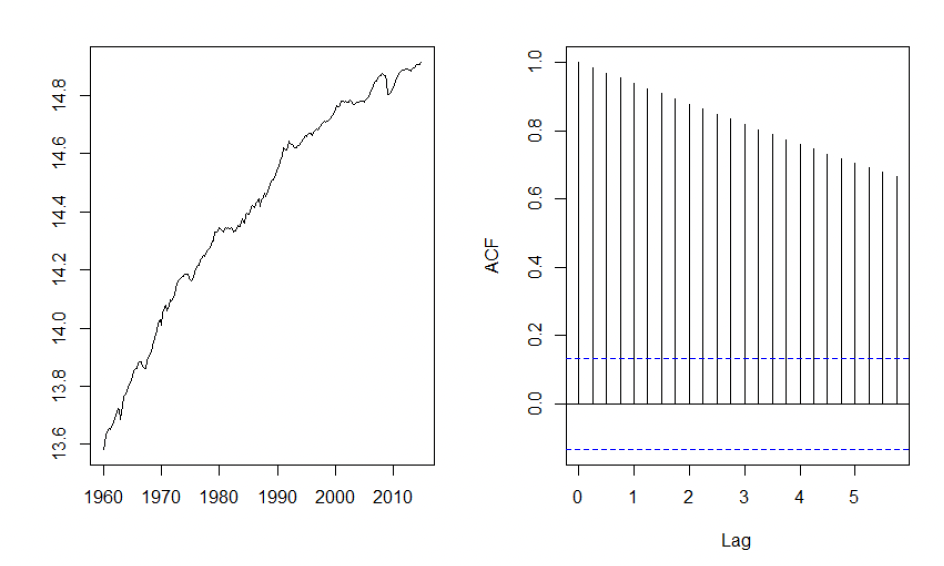
\includegraphics[width=1\linewidth]{Capture d’écran 2025-10-14 à 22.23.30.png}
    \caption{Log of the German GDP and its ACF}
\end{figure}
\end{frame}

% ——————————————————————————————————————————
% Transition to stationarity
% ——————————————————————————————————————————

\section{Stationarity}

\begin{frame}{Non-independence but what about identically distributed?}
\vfill
\centering
\Large
\textit{→ If variables are dependent, can they still be identically distributed?}
\vfill
\end{frame}


% ——————————————————————————————————————————
% Stationarity introduction (Doz)
% ——————————————————————————————————————————

\begin{frame}{Stationary processes}
\small
\begin{itemize}
    \item As only \textbf{one trajectory} of the process $(X_t)_{t \in \mathbb{Z}}$ is observed (corresponding to one realization of nature),
    it is possible to do statistics only if this process exhibits certain regularity properties.
    \vspace{0.3cm}
    \item These regularity properties are called \textbf{stationarity of order 2} (or \textbf{weak stationarity}) properties.
    \vspace{0.3cm}
    \item In the first classes, we will assume $E(X_t^2) < \infty$ and work with processes that are stationary at order 2.
\end{itemize}
\end{frame}




% ——————————————————————————————————————————
% Stationarity definitions
% ——————————————————————————————————————————

\begin{frame}{Definition - Strong Stationarity}
\small
\begin{block}{Definition}
A process $(X_t)_{t \in \mathbb{Z}}$ is defined to be \textbf{strongly stationary} if  
for all $t_1, \ldots, t_n \in \mathbb{Z}$, for all $k \in \mathbb{Z}$ and $n = 1, 2, \ldots$,  
the distribution of the vector $(X_{t_1}, \ldots, X_{t_n})$  
is equal to the distribution of $(X_{t_1 + k}, \ldots, X_{t_n + k})$,  
i.e. all finite-dimensional distributions are identical.
\end{block}
\end{frame}


\begin{frame}{Definition - Weak Stationarity}
\small
\begin{block}{Definition}
A second-order process $(X_t)_{t \in \mathbb{Z}}$ is defined to be \textbf{weakly stationary} if:
\begin{itemize}
    \item[(i)] The mean of the process is constant over time  
    \[
    \text{i.e. } \forall t \in \mathbb{Z}, \quad E(X_t) = \mu.
    \]
    \item[(ii)] The covariance of the process is constant over time  
    \[
    \text{i.e. } \forall t \in \mathbb{Z}, \forall k \in \mathbb{Z}, \quad \gamma(k) = \mathrm{Cov}(X_t, X_{t+k})
    \text{ depends only on } k.
    \]
\end{itemize}
\end{block}
\end{frame}

\begin{frame}{2 kinds of stochastic process}
\begin{figure}
    \centering
    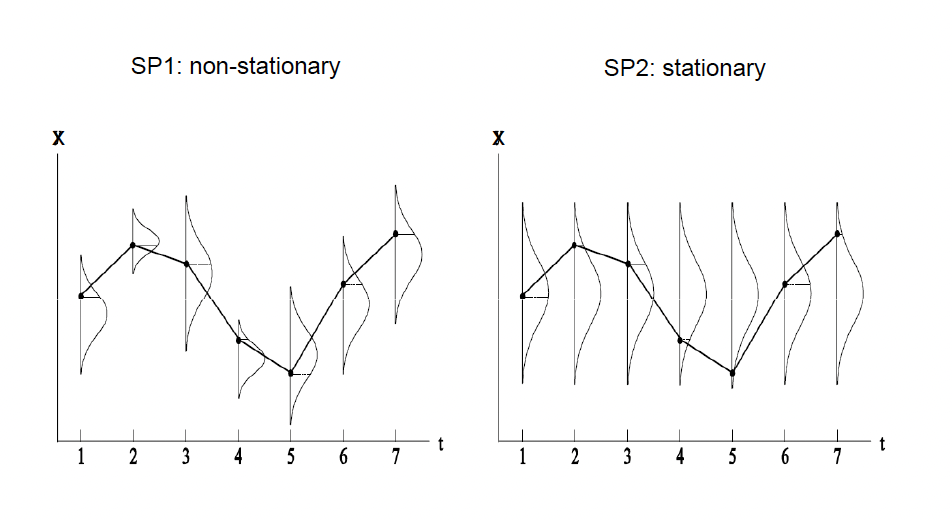
\includegraphics[width=1\linewidth]{Capture d’écran 2025-10-14 à 22.20.04.png}
    
    \label{fig:placeholder}
\end{figure}
\end{frame}




\begin{frame}{Weak vs Strong Stationarity}
\small
\begin{itemize}
    \item A weakly stationary process is also called a \textbf{second-order}, \textbf{covariance} or simply \textbf{stationary} process.
    \vspace{0.2cm}
    \item If a process is stationary, its mean is constant and can be estimated by the empirical mean $\bar X_T$.  
    Hence, we can center any stationary process by subtracting its empirical mean:
    \[
    X_t - \bar X_T.
    \]
\end{itemize}

\vspace{0.3cm}
\begin{block}{Remark}
A strongly stationary process is weakly stationary, but the reverse is not necessarily true.  
An important exception is the \textbf{Gaussian process}, for which both notions coincide.
\end{block}
\end{frame}








% ——————————————————————————————————————————
% Example 1: White Noise
% ——————————————————————————————————————————

\begin{frame}{Example 1 - White Noise}
\small
Let $(X_t)_{t \in \mathbb{Z}}$ be a \textbf{white noise} if:
\begin{itemize}
    \item $\forall t \in \mathbb{Z}, \quad \mathbb{E}(X_t) = 0$
    \item $\forall t \in \mathbb{Z}, \quad \mathbb{V}(X_t) = \sigma^2$
    \item $\forall t, s \in \mathbb{Z}, \; t \neq s \Rightarrow \mathrm{Cov}(X_t, X_s) = 0$
\end{itemize}

\textbf{Notations:}
\begin{itemize}
    \item This is written as $X_t \sim WN(0, \sigma^2)$ or $X_t \rightsquigarrow WN(0, \sigma^2)$.
    \item White noises are often denoted $(\varepsilon_t)_{t \in \mathbb{Z}}$.
\end{itemize}
\end{frame}

\begin{frame}{White Noise ACF}
    \begin{figure}
        \centering
        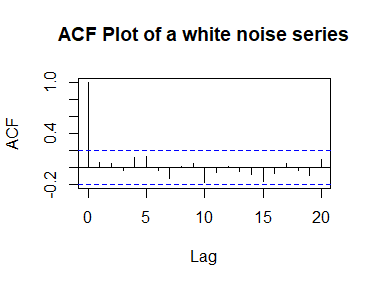
\includegraphics[width=1\linewidth]{wnacf.png}
    \end{figure}
\end{frame}

% ——————————————————————————————————————————
% Example 2: Random Walk (non-stationary)
% ——————————————————————————————————————————

\begin{frame}{Example 2 - Non-stationary process: the Random Walk}
\small
If $\varepsilon_t \sim WN(0, \sigma^2)$ and $(X_t)_{t \in \mathbb{Z}}$ is defined by:
\[
\forall t > 0, \quad X_t = \mu + X_{t-1} + \varepsilon_t, 
\qquad \text{and } \mathrm{Cov}(\varepsilon_t, X_0) = 0,
\]
then $(X_t)_{t \in \mathbb{Z}}$ is a \textbf{random walk}:
\begin{itemize}
    \item with drift if $\mu \neq 0$
    \item without drift if $\mu = 0$
\end{itemize}

\textbf{In both cases,} $(X_t)_{t \in \mathbb{Z}}$ is non-stationary, since:
\[
X_t = X_0 + \mu t + \sum_{s=1}^t \varepsilon_s
\qquad \text{and} \qquad
\mathbb{V}(X_t) = \mathbb{V}(X_0) + t\sigma^2.
\]

\textbf{Remarks:}
\begin{itemize}
    \item If $\mu = 0$, $(X_t)$ is stationary in expectation but not in variance.
    \item If $\mu \neq 0$, $\mathbb{E}(X_t) = \mathbb{E}(X_0) + \mu t$ and $\mathbb{V}(X_t) = t\sigma^2$.
    \item This differs from a process \textbf{stationary around a deterministic trend}:
    \[
    X_t = a + bt + Y_t, \quad \text{where } (Y_t)_{t \in \mathbb{Z}} \text{ is stationary.}
    \]
\end{itemize}
\end{frame}


\begin{frame}{Random Walk}
\begin{figure}
    \centering
    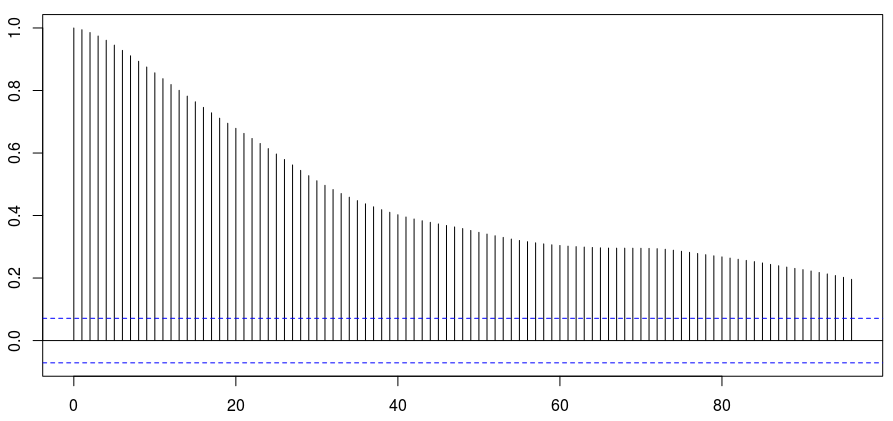
\includegraphics[width=1\linewidth]{rwacf.png}
\end{figure}
    
\end{frame}


\begin{frame}{Random walk with drift vs Trend-stationary process}
\begin{figure}
    \centering
    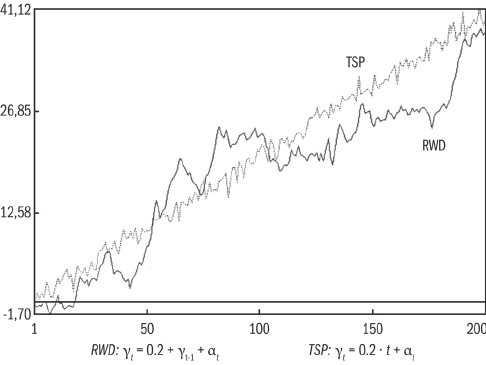
\includegraphics[width=1\linewidth]{rwdd.png}
\end{figure}
\end{frame}

\begin{frame}{}
    \begin{figure}
        \centering
        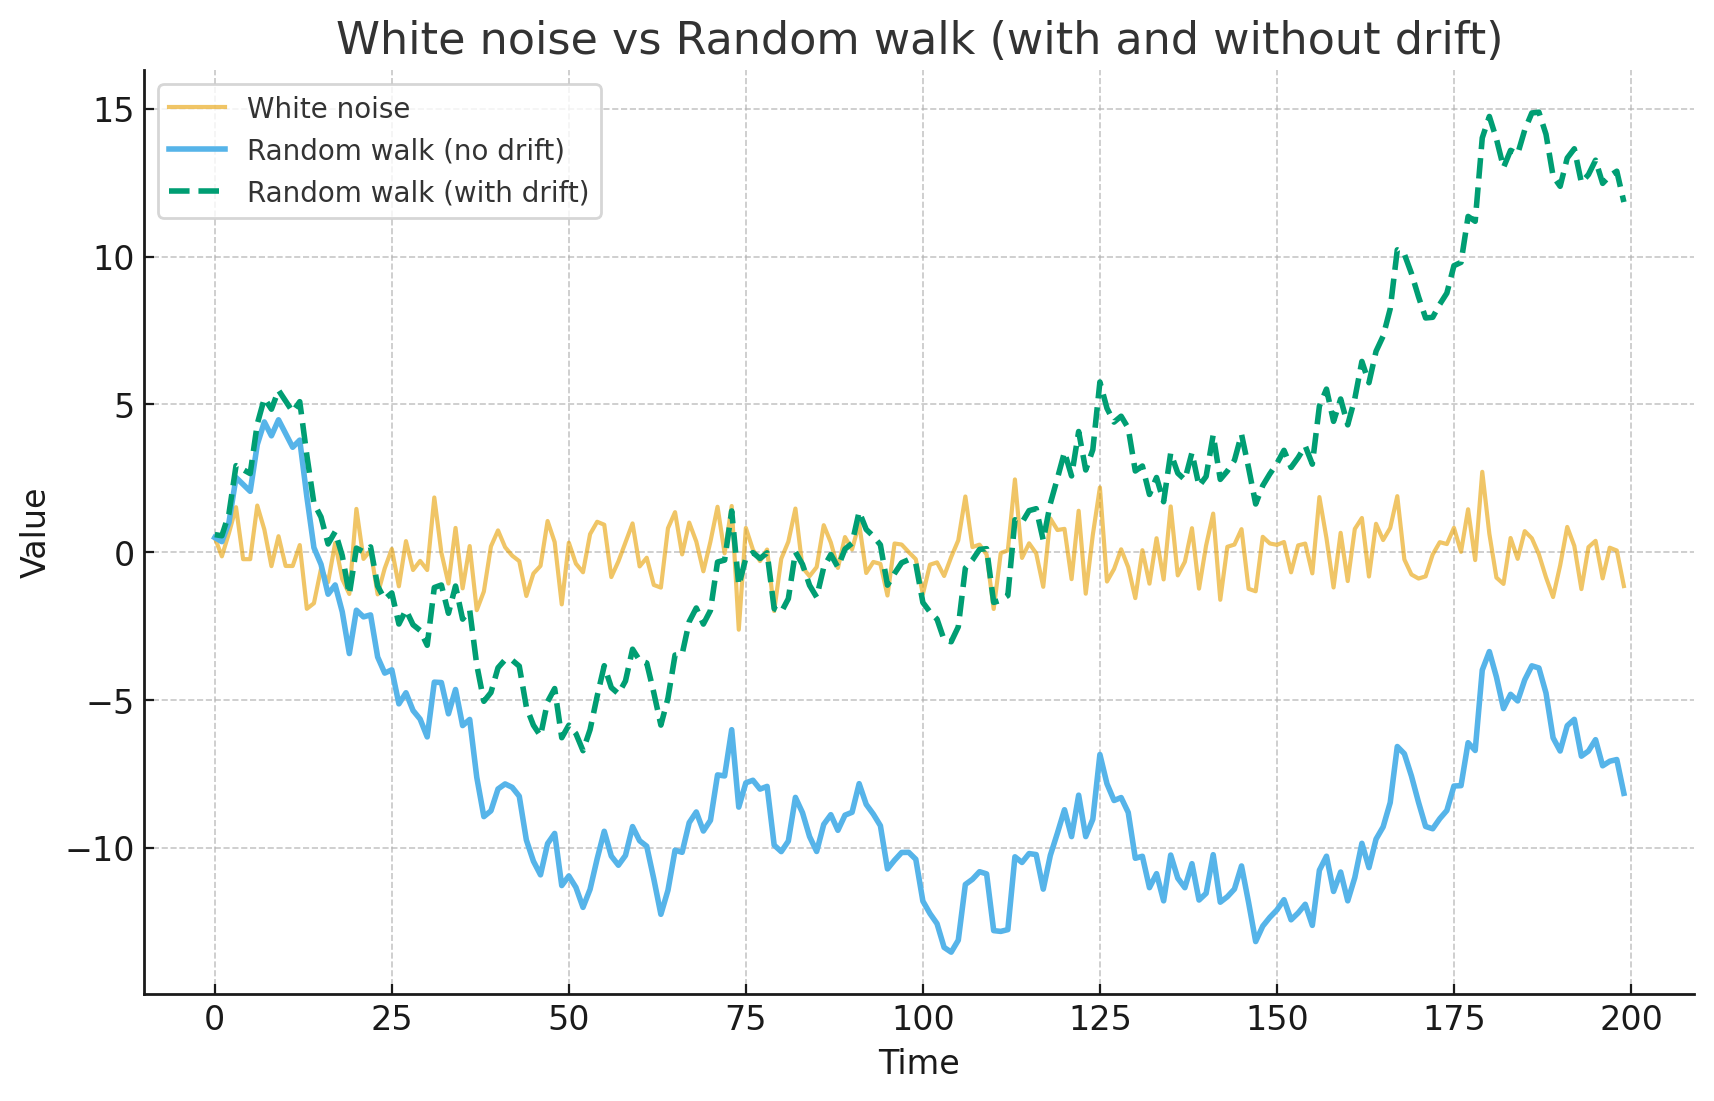
\includegraphics[width=1\linewidth]{comprw.png}
    \end{figure}
\end{frame}



\begin{frame}{NB: Why a Random Walk Does Not Converge (Even with Mean-Zero Shocks)}
\small
\textbf{AR(1) with $\phi = 1$:} 
\[
X_t = X_{t-1} + \varepsilon_t, \quad \varepsilon_t \sim WN(0,\sigma^2)
\]
\[
\Rightarrow X_t = X_0 + \sum_{j=1}^{t} \varepsilon_j
\]

\begin{itemize}
  \item $E[\varepsilon_t] = 0 \ \Rightarrow\ E[X_t] = E[X_0]$ (no drift in mean; if drift: $E[X_t]=E[X_0]+t\beta$)
  \item $\text{Var}(X_t) = t\sigma^2$ (variance grows $\Rightarrow$ nonstationary)
  \item $\displaystyle \frac{1}{t}\sum_{j=1}^{t}\varepsilon_j \xrightarrow{p} 0$ (Law of Large Numbers)
  \item But $\displaystyle \sum_{j=1}^{t}\varepsilon_j = O_p(\sqrt{t})$ (fluctuations accumulate)
\end{itemize}

\textbf{Intuition: "Drunkard’s Walk"}

Each step is centered on 0, but random shocks add up.  
$\Rightarrow$ Average step $\to 0$, yet position \emph{wanders without bound.}
\end{frame}


% ——————————————————————————————————————————
% Why we want stationarity
% ——————————————————————————————————————————
\begin{frame}{Why do we want stationarity?}
\small
\begin{itemize}
  \item \textbf{Ergodicity / identification from one path:} with time-invariant moments, sample averages from a single trajectory consistently estimate population moments.
  \item \textbf{Valid inference:} LLN/CLT apply when mean/variance/covariances do not drift $\Rightarrow$
        OLS/MLE are consistent and asymptotically normal (e.g. $Z'Z/T \to Q$).
  \item \textbf{Stable dependence:} a fixed ACF/PACF makes the \emph{structure of persistence} time-invariant; Wold $\Rightarrow$
   \textbf{     linear representation with innovations = AR, MA, ARMA...!}
  \item \textbf{Forecastability:} parameters and shock variances are constant over time, so models estimated on the past
        remain informative for the future.
  \item \textbf{Practice:} if data are not stationary, \emph{transform} (log, detrend, difference) until the working series is.
\end{itemize}
\end{frame}


% ——————————————————————————————————————————
% Econometric relevance of stationarity
% ——————————————————————————————————————————

\begin{frame}{Why stationarity matters?}
\small
\textbf{Remark:} the stationarity vs non-stationarity issue is crucial beyond Time Series Analysis (without stationarity: no constant mean $E(X_t)$, no stable estimated parameters (can't forecast), invalid inference (can't build a distribution of parameters)...)

\begin{itemize}
    \item Consider a simple econometric model with time series:
    \[
    y_t = a + b x_t + c x_{t-1} + \varepsilon_t = z_t' \beta + \varepsilon_t,
    \quad \varepsilon_t \sim WN(0, \sigma^2).
    \]
    \item In matrix form: \quad $y = Z\beta + \varepsilon$.
    \item If $\dfrac{Z'Z}{T} \xrightarrow{P} Q$, then asymptotic results (LLN, CLT) are valid.
\end{itemize}

\vspace{0.2cm}
\textbf{Here:}
\[
\frac{Z'Z}{T} =
\begin{pmatrix}
\frac{1}{T}\sum x_t^2 & \frac{1}{T}\sum x_t x_{t-1} \\
\frac{1}{T}\sum x_t x_{t-1} & \frac{1}{T}\sum x_{t-1}^2
\end{pmatrix}.
\]

\begin{itemize}
    \item If $(x_t)_{t \in \mathbb{Z}}$ is stationary, this converges in probability to a limit (LLN).
\end{itemize}
\end{frame}



% ——————————————————————————————————————————
% Stationarity vs Ergodicity (for convergence of estimators)
% ——————————————————————————————————————————
\begin{frame}{Stationarity vs Ergodicity (for convergence of estimators)}
\footnotesize
\textbf{Weak stationarity:} $E(X_t)=\mu$, $\mathrm{Var}(X_t)=\sigma^2$, $\mathrm{Cov}(X_t,X_{t-h})=\gamma(h)$ are time-invariant.\\
\textbf{Ergodicity:} time averages reproduce ensemble averages:
\[
\frac{1}{T}\sum_{t=1}^T X_t \xrightarrow{a.s.} E[X_t].
\]
\pause

\begin{itemize}
  \item \textbf{Key link:} Ergodicity is a property defined \emph{within} the class of stationary processes - it is \emph{not} a consequence of stationarity.
        \textbf{Stationarity does not imply ergodicity.}\footnote{\tiny Counter-example: let $Z\sim\mathrm{Bernoulli}(1/2)$ be a fixed (once-drawn) r.v.\ and set $X_t=Z$ for all $t$. This process is stationary ($E[X_t]=1/2$, $\gamma(h)=1/4$ for all $h$), yet its time average equals $Z\neq 1/2$ a.s.: \emph{stationary but not ergodic.}}\\
        Stationarity $+$ \textbf{weak dependence} (mixing or $\sum_h |\gamma(h)|<\infty$) $\Rightarrow$ ergodicity.
  \item \textbf{Main implication:} ensures \textbf{consistency of empirical moments:}
\[
  \bar X_T \xrightarrow{P} \mu,\quad 
  \hat\gamma(h) \xrightarrow{P} \gamma(h),\quad 
  \hat\rho(h) \xrightarrow{P} \rho(h).
  \]
  \item \textbf{Econometric relevance:} in regressions $y_t = z_t'\beta + \varepsilon_t$, ergodicity of $(z_t)$ and $(\varepsilon_t)$ implies  $\frac{Z'Z}{T}\xrightarrow{P}Q$, $\frac{Z'\varepsilon}{T}\xrightarrow{P}0$  
        $\Rightarrow$ \textbf{OLS consistent.}
  \item \textbf{Practical message:} we \emph{assume} stationarity and \emph{require} ergodicity so that inference from one observed path is valid -  i.e. estimators converge as $T \to \infty$.
\end{itemize}
\end{frame}




% ——————————————————————————————————————————
% 3.2 Autocovariance and autocorrelation of a stationary process
% ——————————————————————————————————————————

\begin{frame}{Autocovariance and autocorrelation of a stationary process}
\small
If $(X_t)_{t \in \mathbb{Z}}$ is a stationary process, then:
\begin{itemize}
    \item $\forall h \in \mathbb{Z}$, $\gamma(h) = \gamma(-h)$ :  
    the autocovariance function is \textbf{even}.
    \item $\forall h \in \mathbb{Z}$, 
    \[
    \mathrm{Corr}(X_t, X_{t-h}) = 
    \frac{\mathrm{Cov}(X_t, X_{t-h})}
         {\sqrt{\mathbb{V}(X_t)\mathbb{V}(X_{t-h})}}
    = \frac{\gamma(h)}{\gamma(0)}.
    \]
\end{itemize}

In this case $\mathrm{Corr}(X_t, X_{t-h})$ is denoted as $\rho(h)$, and:
\begin{itemize}
    \item $\forall h \in \mathbb{Z}$, $|\rho(h)| \le 1$;
    \item the function $h \mapsto \rho(h)$ is the \textbf{autocorrelation function};
    \item $\rho$ is an even function;
    \item the graph of $\rho$, for $h \ge 0$, is the \textbf{autocorrelogram}.
\end{itemize}
\end{frame}


% ——————————————————————————————————————————
% 3.5 Empirical moments of stationary processes
% ——————————————————————————————————————————

\begin{frame}{Empirical moments of stationary processes}
\small
The following estimators of theoretical moments are defined:

\begin{itemize}
    \item \textbf{Empirical mean:}
    \[
    \hat m = \bar X_T = \frac{1}{T}\sum_{t=1}^T X_t
    \]
    \item \textbf{Empirical variance:}
    \[
    \hat \gamma(0) = \frac{1}{T}\sum_{t=1}^T (X_t - \bar X_T)^2
    \]
    \item \textbf{Empirical autocovariance of order $h$:}
    \[
    \hat \gamma(h) = \frac{1}{T} \sum_{t=h+1}^T (X_t - \bar X_T)(X_{t-h} - \bar X_T)
    \quad \text{(avoid too large $h$ relative to $T$)}
    \]
    \item \textbf{Empirical autocorrelation:}
    \[
    \hat \rho(h) = \frac{\hat \gamma(h)}{\hat \gamma(0)}
    \]
    \end{itemize}
\end{frame}


% ——————————————————————————————————————————
% Asymptotic properties of empirical moments
% ——————————————————————————————————————————

\begin{frame}{Asymptotic properties of empirical moments}
\small
When $(X_t)_{t \in \mathbb{Z}}$ is stationary, all these estimators are \textbf{consistent}:
\[
T \to \infty \Rightarrow
\begin{cases}
\hat m \xrightarrow{P} m, \\
\hat \gamma(h) \xrightarrow{P} \gamma(h), \\
\hat \rho(h) \xrightarrow{P} \rho(h).
\end{cases}
\]

\vspace{0.3cm}
Moreover, if $(X_t)$ is stationary, the empirical mean is \textbf{asymptotically Gaussian}:
\[
\sqrt{T}(\hat m - m) \xrightarrow{d} \mathcal{N}\!\left(0, \sum_{h \in \mathbb{Z}} \gamma_X(h)\right)
\]
where $\sum_{h \in \mathbb{Z}} \gamma_X(h)$ is called the \textbf{long-run variance}.
\end{frame}



\begin{frame}{Types of Nonstationarity}
\small
Nonstationarity can stem from different sources:

\begin{itemize}
  \item \textbf{Deterministic trends:} predictable changes in mean over time.
  \[
  X_t = a + bt + Y_t, \quad Y_t \text{ stationary.}
  \]
  Example: long-run growth in GDP.

\item \textbf{Seasonality} (because $E(X_t)$ changes along time): periodic deterministic component, often removed by seasonal differencing ($X_t-S_t$).

  \item \textbf{Stochastic trends:} accumulation of random shocks.
  \[
  X_t = X_{t-1} + \varepsilon_t.
  \]
  Example: asset prices on stock markets, productivity shocks (innovation).

  \item \textbf{Structural breaks:} discrete changes in mean, variance (heteroskedasticity) or dynamics (e.g. regime-dependent).

\end{itemize}

\end{frame}


\begin{frame}{Types of Nonstationarity}

\textbf{Goal:} Determine whether nonstationarity comes from a deterministic or stochastic source.  
\medskip
\textbf{Example:} the \textit{Great Moderation} (mid-1980s): a major decline in macroeconomic volatility, often attributed to changes in monetary policy and inventory behavior
\medskip
(actually \textbf{NO} - "Is the Stabilization of the Postwar U.S. Economy a Figment of the Data?", Christina Romer (AER, 1986), just a question of data construction \& measurement). 
\medskip
\textbf{Tools:} \textbf{visual inspection, ACF, unit-root tests (ADF, KPSS, etc.).}

\end{frame}


\begin{frame}{Trend-Stationary vs Difference-Stationary Processes}
\small
\textbf{Trend-Stationary (TS):}
\[
X_t = a + bt + Y_t, \quad Y_t \text{ stationary.}
\]
After removing the deterministic trend $(a+bt)$, residuals $Y_t$ are stationary.
\medskip
\textbf{Difference-Stationary (DS):}
\[
X_t = X_{t-1} + \varepsilon_t, \quad \Delta X_t = \varepsilon_t \text{ stationary.}
\]
A stochastic trend (unit root) - differencing yields a stationary process.
\medskip
\textbf{Interpretation:}
\begin{itemize}
\item \textbf{TS: shocks are \emph{transitory} - series reverts to deterministic trend.}
\item \textbf{DS: shocks are \emph{permanent} - they shift the level permanently.}
\end{itemize}

\textbf{Practical consequence:}  
Different transformations are needed for stationarization (detrending vs differencing).  
Testing for a unit root helps decide which model fits the data.
\end{frame}


\begin{frame}{}
    \begin{figure}
        \centering
        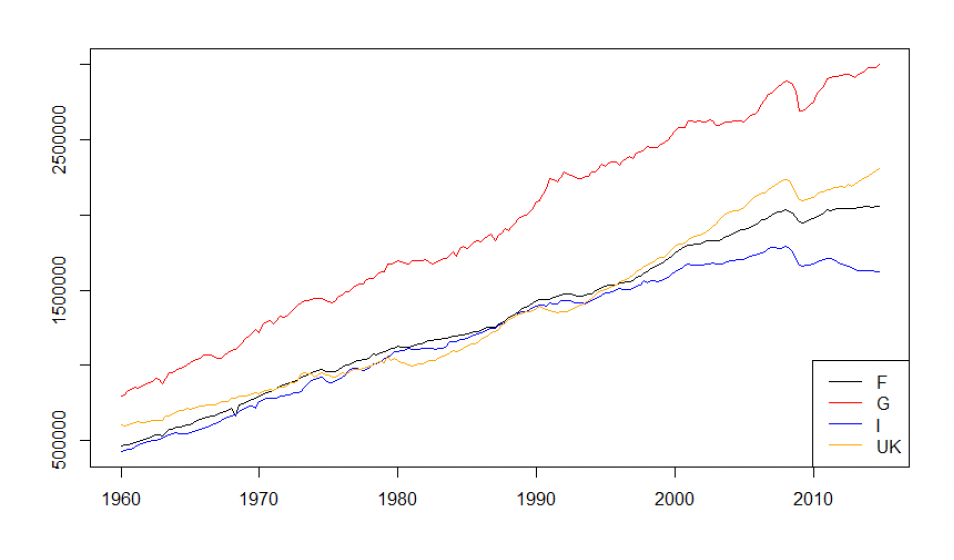
\includegraphics[width=1\linewidth]{Capture d’écran 2025-10-14 à 22.22.10.png}
        \caption{European GDPs}
    \end{figure}
\end{frame}



\begin{frame}{Testing for Unit Roots}
\small
\textbf{Goal:} determine whether nonstationarity stems from a\textbf{ stochastic trend (unit root, thus random walk)} or a \textbf{deterministic trend (drift/linear trend)}.\textit{ 
\medskip
"Does the series tend to return to a fixed mean/trend after a shock, or do shocks accumulate permanently?"}

\vspace{0.3cm}
\begin{itemize}
  \item A \textbf{constant} in the test equation allows for a non-zero mean (level).
  \item A \textbf{trend} allows for a deterministic drift over time.
  \item $\Rightarrow$ Choosing “constant” vs “trend” depends on the data pattern:
  \begin{itemize}
    \item fluctuates around a fixed mean $\to$ include a constant only;
    \item grows/declines linearly over time $\to$ include constant + trend.
  \end{itemize}
\end{itemize}
\end{frame}


\begin{frame}{Testing for Unit Roots}
\small

\begin{enumerate}
  \item \textbf{ADF (Augmented Dickey-Fuller):} classical regression-based test.  
\[
\Delta X_t = \alpha + \beta t + (\phi - 1) X_{t-1} + \sum_{i=1}^{p}\delta_i \Delta X_{t-i} + \varepsilon_t
\]
  $H_0$: unit root (nonstationary, $ (\phi -1) = 0$); $H_1$: stationary ($ (\phi - 1) < 0$).
  
  \item \textbf{PP (Phillips-Perron):} same null as ADF but nonparametric correction for serial correlation (uses long-run variance).

  \item \textbf{DF-GLS (Elliott-Rothenberg-Stock):} more powerful variant - detrends first, then applies DF test.

  \item \textbf{KPSS (Kwiatkowski-Phillips-Schmidt-Shin):} \textbf{\textit{opposite null}.  }
  $H_0$: stationary (around mean or trend); $H_1$: unit root.
\end{enumerate}

\textbf{Practical rule of thumb:}
\begin{itemize}
  \item Reject ADF/PP/DF–GLS $\Rightarrow$ stationary.
  \item Reject KPSS $\Rightarrow$ nonstationary.
  \item Combine both (ADF + KPSS) for robust diagnosis.
\end{itemize}
\end{frame}


%======================================================
\begin{frame}{Unit Root Tests and Structural Breaks}
%======================================================
\footnotesize

\alert{\textbf{Critical caveat:}} ADF, PP, and KPSS have \textbf{near-zero power} when the series is \emph{stationary around a shifted mean or a broken trend}: they systematically conclude unit root in error.

\medskip
\textbf{Three tests for structural breaks:}

\begin{enumerate}
  \item \textbf{Chow (1960):} \emph{known} break date $T_b$. Split sample at $T_b$, test equality of regression coefficients across sub-samples via an $F$-statistic.

  \item \textbf{Perron (1989):} \emph{known} $T_b$. Modified ADF including a shift dummy (level or trend). $H_0$: unit root with break; $H_1$: stationary with break. Avoids confounding a shift in mean/trend with a stochastic trend (vs.\ Chow's shortcomings).

  \item \textbf{Zivot-Andrews (1992):} \emph{unknown} $T_b$. Runs a Perron-type ADF for every candidate break date; selects $T_b$ as the date minimising the $t$-statistic on the unit-root coefficient. Critical values are adjusted for the data-mining.%
  \footnote{\scriptsize \textbf{Bai-Perron (1998)} extends to \emph{multiple} unknown breaks.}
\end{enumerate}

\medskip
\textbf{Practical rule:}
\begin{itemize}
  \item Inspect visually for level shifts or trend changes (crisis, policy regime change, war\dots).
  \item If suspected, apply Zivot-Andrews \emph{before} concluding $I(1)$.
  \item A series may appear $I(1)$ purely because of an unmodelled break.
\end{itemize}
\end{frame}


% Slide 1
\begin{frame}{Structural Break vs. Stochastic Trend}

\centering
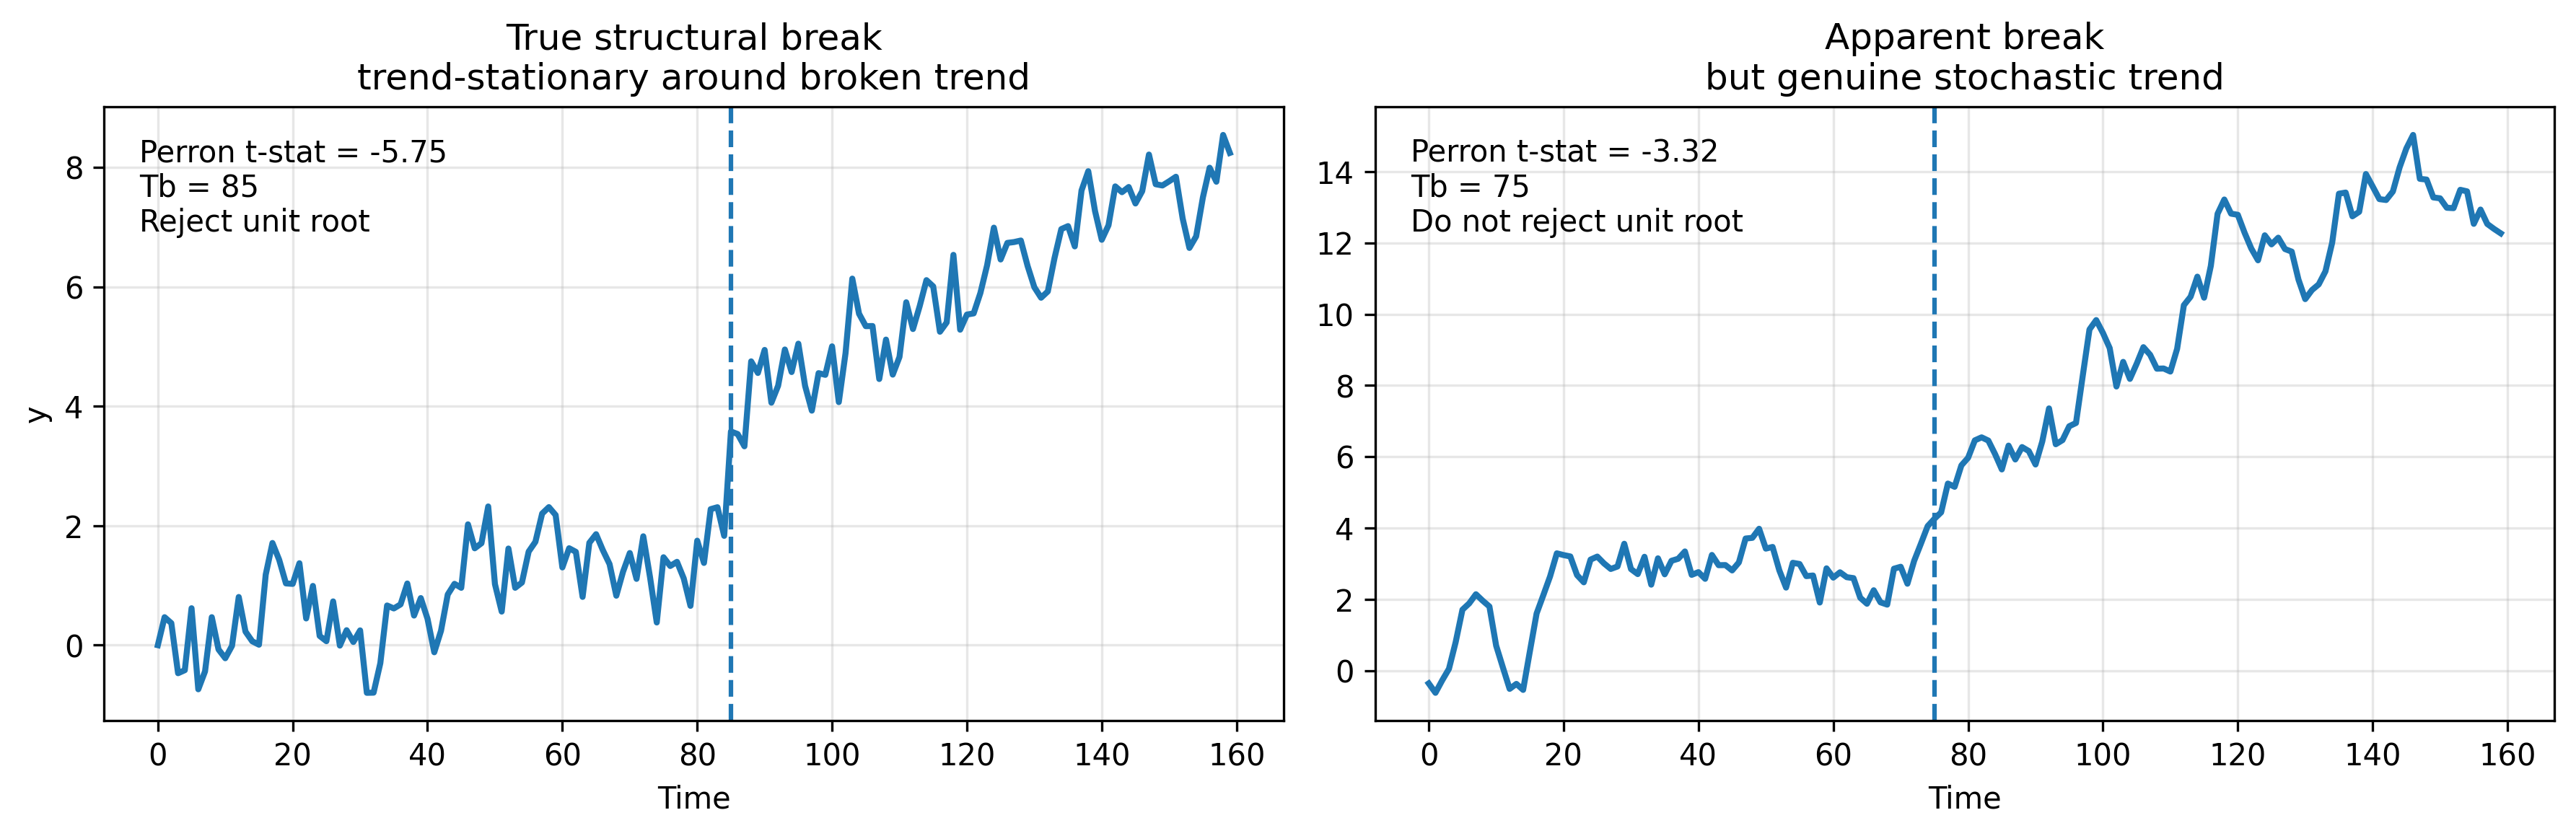
\includegraphics[width=1\textwidth]{image/structural_break_vs_stochastic_trend.png}

\end{frame}


% Slide 2
\begin{frame}{Perron Test: Interpretation}

\textbf{Perron-type ADF test with known break date}

\medskip

\begin{itemize}
  \item \textbf{Left series: true deterministic structural break}
  \begin{itemize}
    \item Break date: $T_b = 85$
    \item Test statistic: $-5.751$
    \item Approx. 5\% critical value: $-5.08$
    \item Since $-5.751 < -5.08$, we reject the unit-root null.
    \item Interpretation: the series is trend-stationary around a broken deterministic trend.
  \end{itemize}

  \medskip

  \item \textbf{Right series: genuine stochastic trend}
  \begin{itemize}
    \item Candidate break date: $T_b = 75$
    \item Test statistic: $-3.320$
    \item Approx. 5\% critical value: $-5.08$
    \item Since $-3.320 > -5.08$, we do not reject the unit-root null.
    \item Interpretation: the apparent break does not remove the stochastic trend.
  \end{itemize}
\end{itemize}

\medskip

\textbf{Takeaway:} a deterministic break can mimic a unit root, but a genuine stochastic trend can also mimic a break.

\end{frame}

\begin{frame}{Making Series Stationary}
\small
Once nonstationarity is detected, we can apply transformations to stabilize mean and variance:

\begin{enumerate}
  \item \textbf{Logarithm:} removes exponential growth and stabilizes variance.
  \item \textbf{Detrending (OLS):} removes deterministic trend components.
  \item \textbf{Differencing:} removes stochastic trends or unit roots.
  \item \textbf{Filtering:} removes low-frequency components (e.g. HP, BK, CF filters).
\end{enumerate}

\pause
\textbf{Empirical workflow:}
\begin{enumerate}
  \item Visual inspection: guess the type of trend.
  \item Unit root tests
  \item Apply the appropriate transformation.
  \item Test residuals for stationarity (ACF tail decay, formal tests).
\end{enumerate}


\end{frame}

\section{Transformations}

% ——————————————————————————————————————————
% Deseasonalization Methods (Pedagogical slide)
% ——————————————————————————————————————————
\begin{frame}{Removing Seasonality (Deseasonalization)}
\footnotesize

\textbf{Goal:} eliminate the recurring seasonal pattern $s_t$ so that the residual series
has a constant mean and time-invariant covariance.

\vspace{0.2cm}
\textbf{Two main approaches:}

\vspace{0.3cm}
\begin{block}{(a) Deterministic seasonality -Regression on seasonal dummies}
\begin{itemize}
  \item Assume a fixed, repeating seasonal pattern (e.g. same months or quarters every year):
  \[
  X_t = \alpha + \sum_{m=1}^{S-1}\beta_m D_{m,t} + u_t,
  \quad D_{m,t}=1 \text{ if period } m, \; 0 \text{ otherwise.}
  \]
  \item The fitted part $\hat\alpha + \sum \hat\beta_m D_{m,t}$ captures seasonality.
  \item \textbf{Deseasonalized series:}
  \[
  X_t^* = X_t - \big(\hat\alpha + \sum_{m=1}^{S-1}\hat\beta_m D_{m,t}\big).
  \]
\end{itemize}
\textit{Works well when the seasonal pattern is stable over time.}
\end{block}
\end{frame}


\begin{frame}{Removing Seasonality (Deseasonalization)}
\begin{block}{(b) Stochastic or time-varying seasonality - Seasonal differencing}
\begin{itemize}
  \item If the strength of the seasonal effect changes slowly:
  \[
  \Delta_S X_t = X_t - X_{t-S}.
  \]
  \item Example: $\Delta_{12}X_t$ for monthly data removes yearly periodicity.
  \item Since $E[X_t - X_{t-S}] = s_t - s_{t-S} = 0$, the mean becomes constant.
\end{itemize}
\textit{Standard in SARIMA models; keeps short-run dynamics.}
\end{block}
\end{frame}

% ——————————————————————————————————————————
% First transformation: logarithm
% ——————————————————————————————————————————
\begin{frame}{First transformation: logarithm}
\textbf{1st transformation:} $\log(x_t)$

\begin{itemize}
  \item \textbf{Stabilizes variance (level-dependent volatility).} 
  Many macro series grow roughly exponentially meaning their variance increases with their level so taking logs transforms exponential growth into approximately linear growth (turns multiplicative growth into additive changes) making fluctuations more homoscedastic and models better behaved.
  \item \textit{Interpretability:} log-differences approximate percentage growth (cf. infra!)
\end{itemize}
\end{frame}



\begin{frame}{First transformation: logarithm}
    \begin{figure}
        \centering
        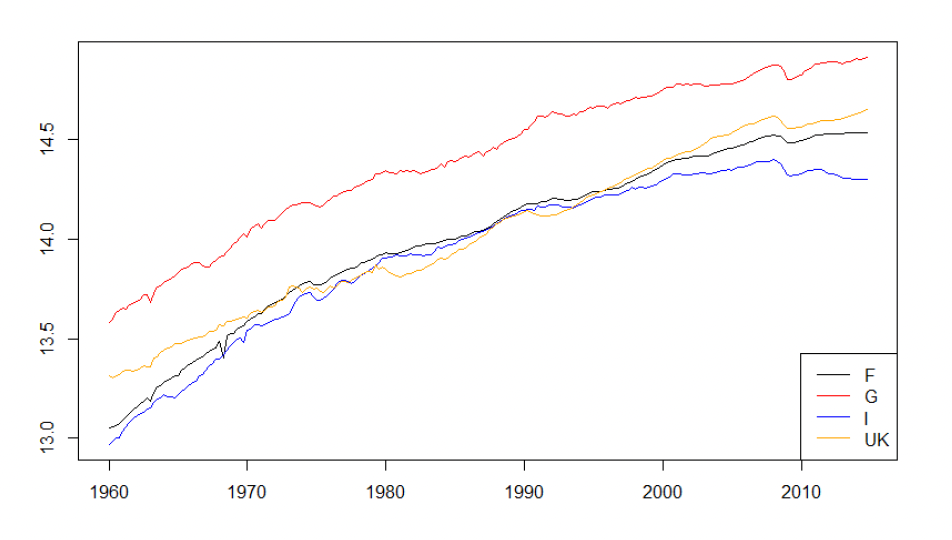
\includegraphics[width=1\linewidth]{Capture d’écran 2025-10-14 à 22.23.01.png}
        \caption{European GDPs : logarithm}
    \end{figure}
\end{frame}



\begin{frame}{First transformation: logarithm}
\begin{figure}
    \centering
    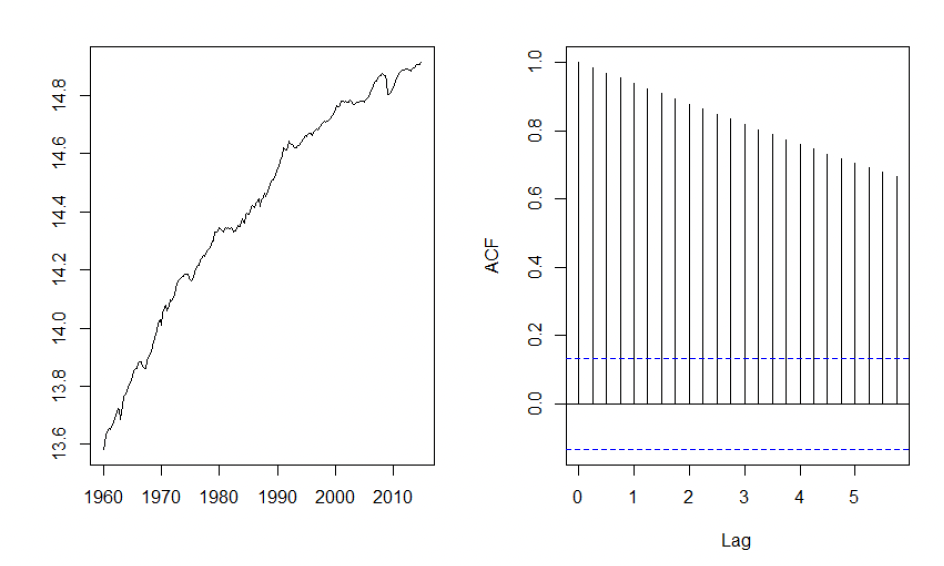
\includegraphics[width=1\linewidth]{Capture d’écran 2025-10-14 à 22.23.30.png}
    \caption{Log of the German GDP and its ACF}
\end{figure}
\end{frame}



% ——————————————————————————————————————————
% 2nd transformation: deviations from deterministic trends (OLS)
% ——————————————————————————————————————————

\begin{frame}{2nd transformation: Deviations from deterministic trends (OLS)}
\small
\textbf{Idea:} remove the deterministic trend of $\log(x_t)$ estimated by OLS.

\vspace{0.3cm}
\begin{itemize}
    \item \textbf{Linear case:}
    \[
    x_t^{*} = \log(x_t) - \hat{\beta}_0 - \hat{\beta}_1 t
    \]
    \item \textbf{Quadratic case:}
    \[
    x_t^{*} = \log(x_t) - \hat{\beta}_0 - \hat{\beta}_1 t - \hat{\beta}_2 t^2
    \]
\end{itemize}

\vspace{0.2cm}
\textbf{Example:} German GDP

\vspace{0.4cm}
\centering
\textcolor{blue}{\textbf{Table - OLS estimation}}

\vspace{0.2cm}
\begin{tabular}{lccc}
\toprule
\textbf{Trend} & $\hat{\beta}_0$ & $\hat{\beta}_1$ & $\hat{\beta}_2$ \\
\midrule
Linear & 13.78 & 0.005 & -- \\
Quadratic & 13.62 & 0.010 & -0.00002 \\
\bottomrule
\end{tabular}
\end{frame}



\begin{frame}{2nd Transformation}
\begin{figure}
    \centering
    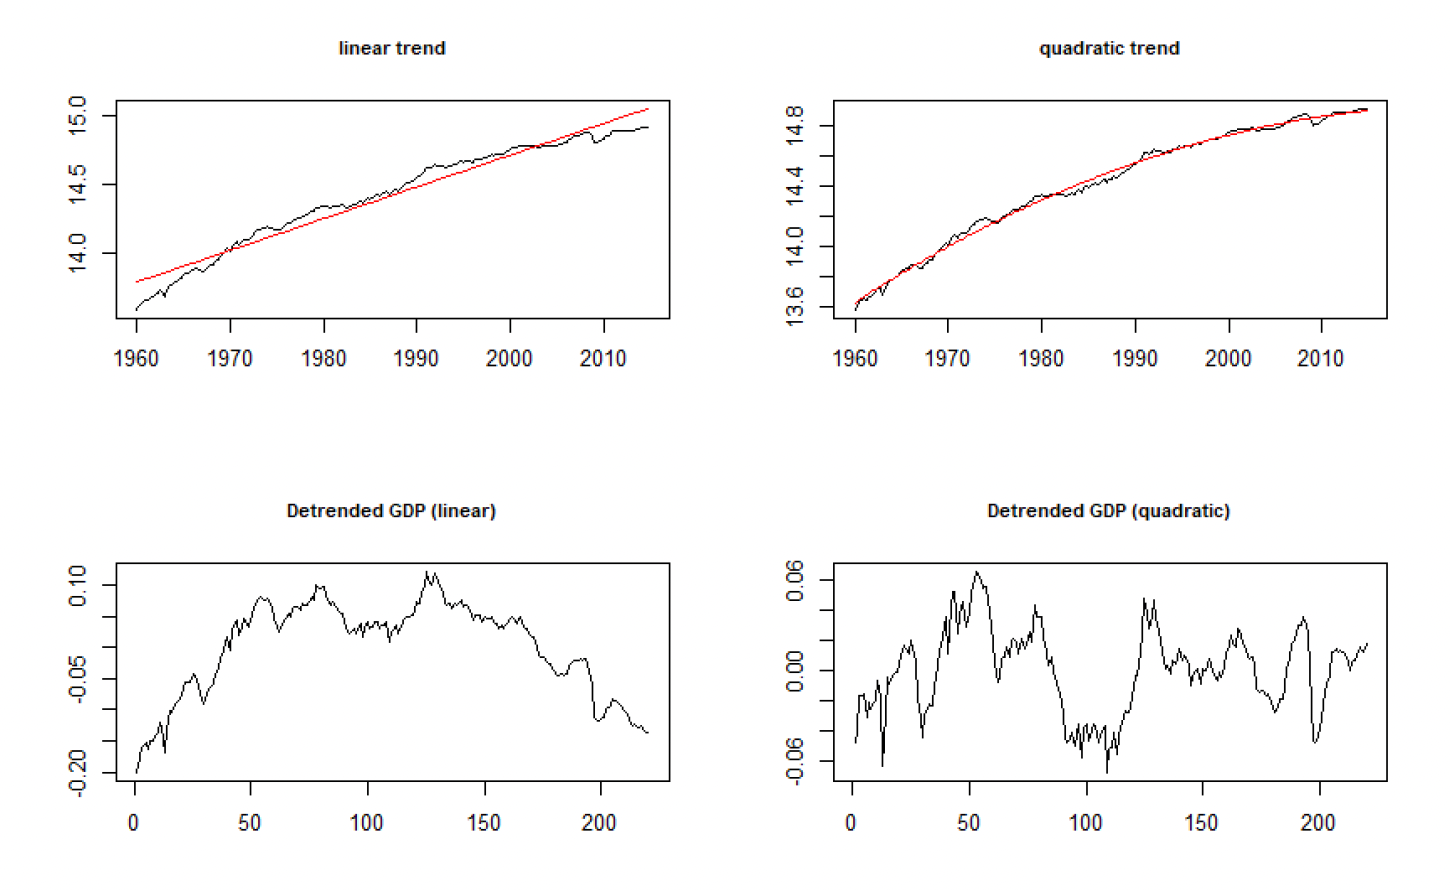
\includegraphics[width=1\linewidth]{Capture d’écran 2025-10-14 à 22.25.37.png}
    \caption{Detrended German GDP (in log) : linear vs quadratic}
\end{figure}
\end{frame}

\begin{frame}{2nd Transformation}
\begin{figure}
    \centering
    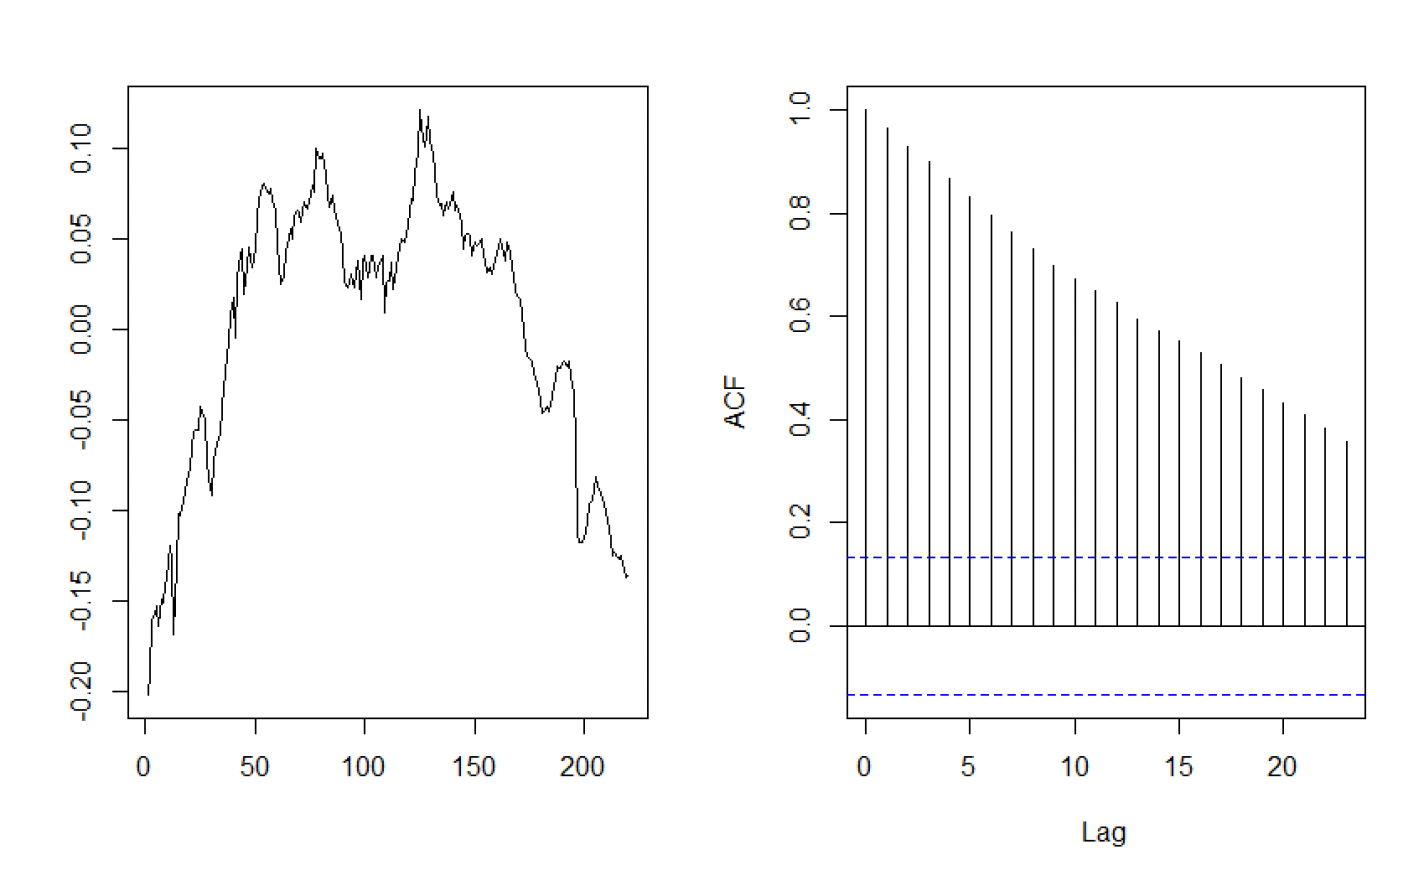
\includegraphics[width=1\linewidth]{Capture d’écran 2025-10-14 à 22.26.07.png}
    \caption{Detrended Log of the German GDP and its ACF : linear version}
\end{figure}
\end{frame}



\begin{frame}{2nd Transformation}
\begin{figure}
    \centering
    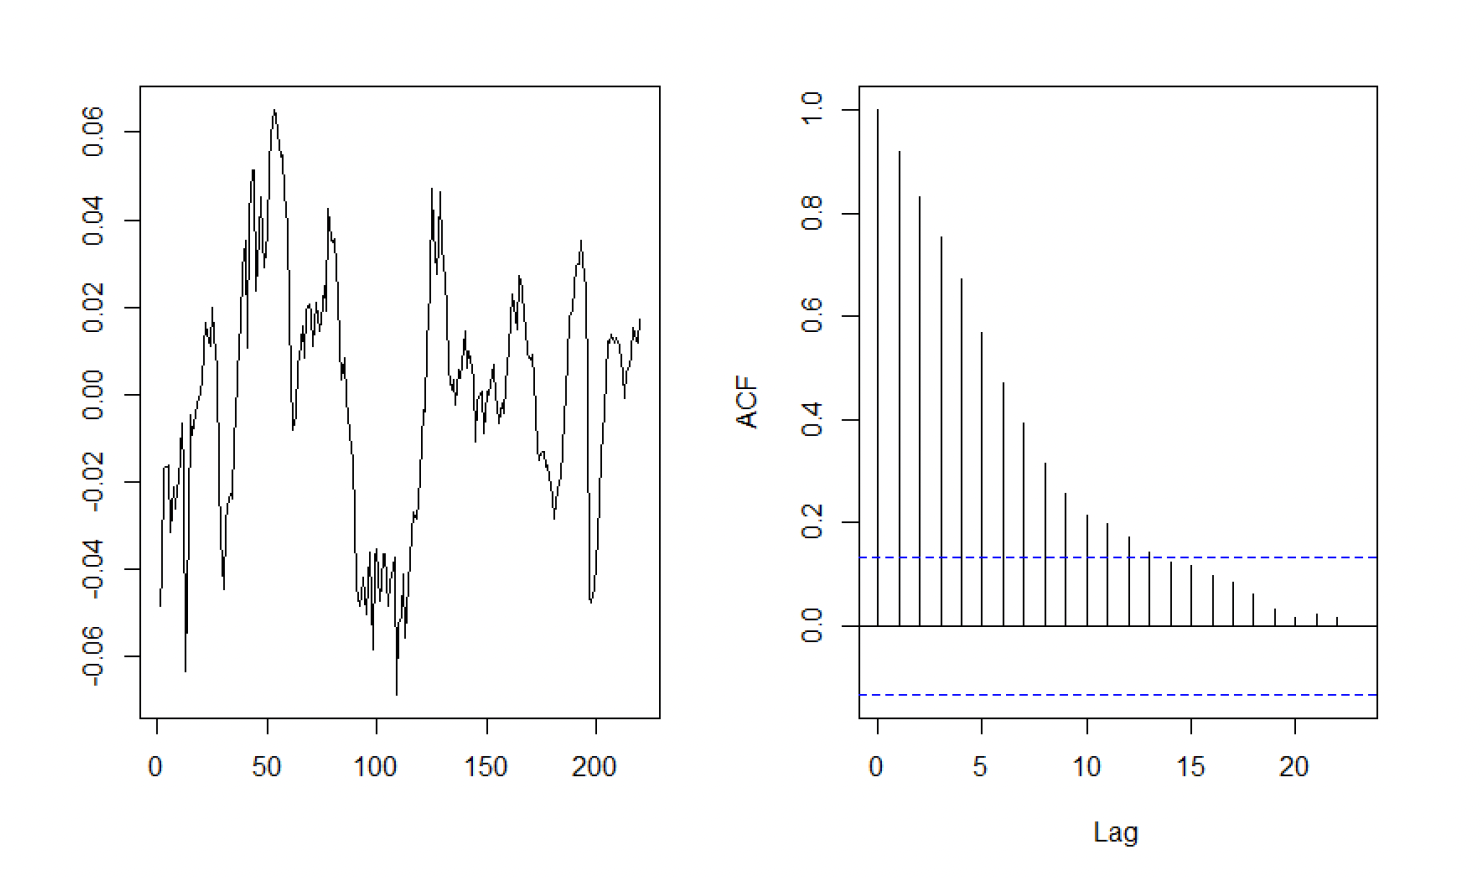
\includegraphics[width=1\linewidth]{Capture d’écran 2025-10-14 à 22.27.07.png}
    \caption{Detrended Log of the German GDP and its ACF : quadratic version}
\end{figure}
\end{frame}


\begin{frame}{3rd transformation, if Random Walk (unit root): First differences}
\small
\textbf{Definition:} first differences in logarithms approximate growth rates.
\[
\Delta \log(x_t) = \log(x_t) - \log(x_{t-1}) \approx \frac{x_t - x_{t-1}}{x_{t-1}}
\]
\pause
\textbf{Proof:}
\[
\begin{aligned}
\Delta \log(x_t) &= \log x_t - \log x_{t-1} = \log \frac{x_t}{x_{t-1}} \\
&= \log\!\left(\frac{x_t}{x_{t-1}} - 1 + 1\right)
  = \log\!\left(\frac{x_t - x_{t-1}}{x_{t-1}} + 1\right)
\end{aligned}
\]

\vspace{0.2cm}
For small relative changes, $\displaystyle \log(1 + \epsilon) \approx \epsilon$, so:
\[
\Delta \log(x_t) \approx \frac{x_t - x_{t-1}}{x_{t-1}}.
\]
\end{frame}

% ——————————————————————————————————————————
% Summary: transformation & stationarity roadmap
% ————————————————————————————
\begin{frame}{Difference between centering and differencing? Removing Trend / Random Walk?}
\small

\textbf{Trend-Stationary (TS):}
\[
X_t = a + bt + Y_t,\quad \mathbb{E}[Y_t]=0,\; Y_t \sim I(0).
\]
\textit{Detrending} $\Rightarrow$ $Y_t$ (stationary \& \textbf{centered on 0}).\\
\textit{Differencing} $\Rightarrow$ $\Delta X_t = b + \Delta Y_t$ with $\mathbb{E}[\Delta X_t]=b$
(\textbf{not centered} otherwise no trend in level (GDP growth rate is centered on > 0, otherwise no long-run growth!). Unless $b=0$).

\medskip
\textbf{Difference-Stationary (Random Walk) with drift $\mu$:}
\[
X_t = \mu + X_{t-1} + \varepsilon_t,\quad \mathbb{E}[\varepsilon_t]=0.
\]
\textit{Differencing} $\Rightarrow$ $\Delta X_t = \mu + \varepsilon_t$ (stationary but \textbf{not centered} unless $\mu=0$).\\
\textbf{Without drift} ($\mu=0$): $\Delta X_t=\varepsilon_t$ (\textbf{centered on 0}).

\medskip
\textbf{Summary:}
\begin{itemize}
  \item TS: detrending $\Rightarrow$ centered on 0; differencing $\Rightarrow$ mean $b$.
  \item RW: differencing $\Rightarrow$ mean $\mu$ (often $>0$ in macro), centered only if $\mu=0$.
\end{itemize}

\end{frame}


\begin{frame}{Summary: Transformations to Achieve Stationarity}
\small
\textbf{Objective:} ensure time-invariant mean, variance, and covariance.

\begin{itemize}
  \item Log-transform $\Rightarrow$ stabilize variance.
  \item Detrending $\Rightarrow$ remove deterministic growth.
  \item Differencing $\Rightarrow$ remove stochastic trends (unit root).
\end{itemize}

\pause
\textbf{Rule of thumb:}
\[
\begin{cases}
x_t^* = x_t - \hat a - \hat b t & \Rightarrow \text{trend-stationary (TS)}\\[4pt]
\Delta x_t = x_t - x_{t-1} & \Rightarrow \text{difference-stationary (DS)}
\end{cases}
\]

\textbf{But:} filters can isolate frequency components rather than parametric trends $\to$ useful for business-cycle analysis, but \textbf{\textit{choice of filter = implicit assumption about what counts as a “cycle.”}}

\medskip
\textbf{If stationary series: \textit{"integrated at order 0"} ($I(0)$).} If need differencing once, integrated order $I(1)$. If d-times, $I(d)$. Any $I(2)$ series? 
\end{frame}

\begin{frame}{From Detrending to Filtering: Two Goals}
\small
\textbf{Detrending} removes deterministic growth $\Rightarrow$ \textit{stationarity}.
\vspace{0.2cm}

\textbf{Filtering} separates movements by \textit{frequency} $\Rightarrow$ \textit{business-cycle extraction.}

\begin{block}{Idea: time series = signal + noise at different frequencies}
\[
X_t = T_t + C_t + \varepsilon_t
\]
\begin{itemize}
  \item $T_t$: slow, low-frequency (long-run trend)
  \item $C_t$: medium frequency (business cycle)
  \item $\varepsilon_t$: high-frequency (noise)
\end{itemize}
\end{block}

\textbf{Goal:} isolate the component relevant for the question.
\begin{itemize}
  \item For forecasting $\Rightarrow$ remove nonstationary trend.
  \item For cyclical analysis $\Rightarrow$ remove high and low frequencies.
\end{itemize}

\textbf{But WHAT is the trend and WHAT is the business cycle???}
\end{frame}


\begin{frame}{Main Filtering Methods}
\small
\textbf{1. Hodrick-Prescott (HP) filter}
\begin{itemize}
  \item Penalizes variability in the trend: $\min_T \sum_t (X_t - T_t)^2 + \lambda \sum_t (\Delta^2 T_t)^2$
  \item $\lambda$ controls smoothness ($\lambda=1600$ quarterly)
  \item Gives $X_t = T_t + C_t$ with $C_t$ stationary
\end{itemize}

\textbf{2. Baxter-King (BK) filter}
\begin{itemize}
  \item Band-pass: isolates frequencies corresponding to cycles of 6-32 quarters.
  \item Symmetric moving average $\to$ introduces edge loss.
  \item And suppress cyclicality if the endogenous dynamics lie actually beyond 32Q (medium-run capacity utilization, longer financial run (credit volumes, leverage etc. à la Borio, BIS). 
\end{itemize}

\textbf{3. Christiano-Fitzgerald (CF) filter}
\begin{itemize}
  \item Similar to BK but optimized for finite samples $\to$ less edge distortion.
\end{itemize}
\end{frame}


\begin{frame}{My work}
\small
What I'm doing right now: \textit{Are Cycles Cyclical? Are macro-financial dynamics endogenous or shock-driven?} Studying "agnostic" ways to separate frequencies. 
\begin{figure}
    \centering
    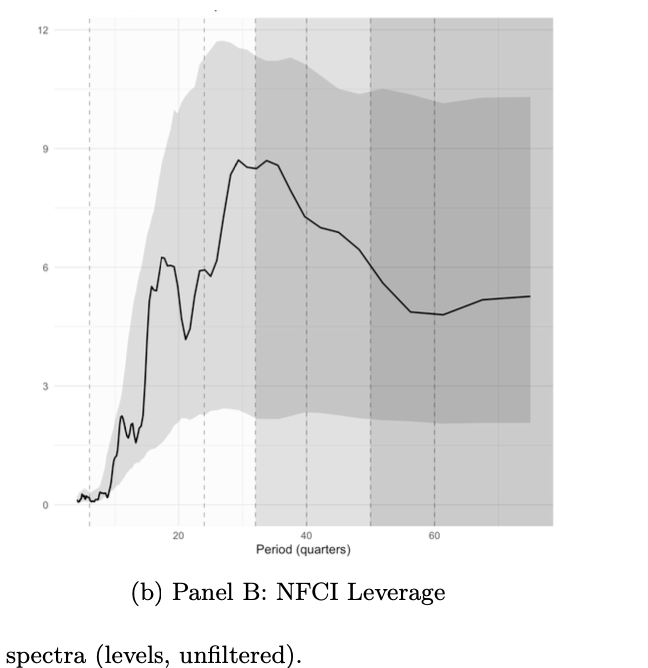
\includegraphics[width=0.5\linewidth]{Capture d’écran 2025-10-22 à 15.40.08.png}
\end{figure}
    \textbf{Detrending methods are usually discretionary and parametric! Direct impact on what is the TREND and what is the CYCLE! }

\end{frame}



\begin{frame}{DETRENDING/FILTERING IS A NON-TRIVIAL ISSUE}
    \centering
  \small
The HP filter can mistake a long slump for a fall in potential output, pulling the “trend” down until the economy seems back at full employment.

Great Depression example: misreads it as lower potential rather than sustained demand shortfall (the filter absorbs the depression into the trend, erasing genuine cyclical slack).

Hamilton (2018) \textit{“Why You Should Never Use the Hodrick-Prescott Filter”}
    
\begin{figure}
    \centering
    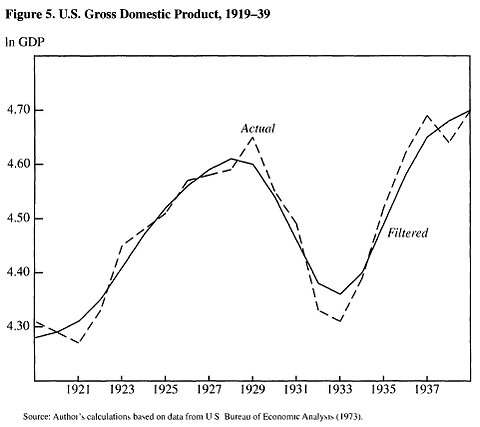
\includegraphics[width=0.5\linewidth]{HP fi.png}
\end{figure}
\end{frame}


% ——————————————————————————————————————————
% Limits of parametric discretionary filters (HP example)
% 


\section{Consequences}
% ——————————————————————————————————————————
% Wold decomposition, linearity and OLS foundation
% ——————————————————————————————————————————
\begin{frame}{From Stationarity to Prediction: Wold Decomposition and Linearity}
\small
\textbf{Wold Decomposition Theorem:}  
Any zero-mean, weakly stationary process $\{X_t\}$ can be written as:
\[
X_t = X_t^{(d)} + X_t^{(s)}, \qquad
X_t^{(s)} = \sum_{j=0}^{\infty} \psi_j \varepsilon_{t-j},
\]
where:
\begin{itemize}
    \item $X_t^{(d)}$ is a \textbf{deterministic} (perfectly linearly predictable) component;
    \item $X_t^{(s)}$ is the \textbf{purely nondeterministic} (stochastic) component driven by uncorrelated innovations
          $\varepsilon_t \sim WN(0,\sigma^2)$, with $\sum_j \psi_j^2 < \infty$.
\end{itemize}

\pause
\textbf{Interpretation:}
\begin{itemize}
    \item The Wold representation describes the \emph{best linear predictor} of $X_t$ from its past.
    \item It ensures that any stationary process can be \emph{approximated} (in mean-square sense)
          by a linear process.
    \item $\Rightarrow$ motivates using \textbf{linear AR, MA, ARMA models} 
\end{itemize}

\textbf{Note:}  
Wold’s theorem does \emph{not} imply that all stationary processes are truly linear (e.g. GARCH, nonlinear Markov chains), only that their second-order structure is linearizable and thus admit a linear representation.
\end{frame}



\begin{frame}{From Stationarity to Prediction: Wold Decomposition and Linearity}
\textbf{Implication for prediction:}
\begin{itemize}
    \item The stationarity property ensures that all non-conditional moments of the predictor $X_{T+h}$  
    (for any $h>0$) can be estimated from $(X_1, \ldots, X_T)$.
    \item Thus, a simple non-conditional predictor is the empirical mean:
    \[
    \hat X_{T+h} = \bar X_T = \frac{1}{T}\sum_{t=1}^T X_t.
    \]
    \item However, this naive predictor is constant for all horizons $h$!
    \item To capture dynamics, we need \textbf{dynamic linear models (AR, MA, ARMA)}.
\end{itemize}
\end{frame}

\begin{frame}{}
\begin{figure}
    \centering
    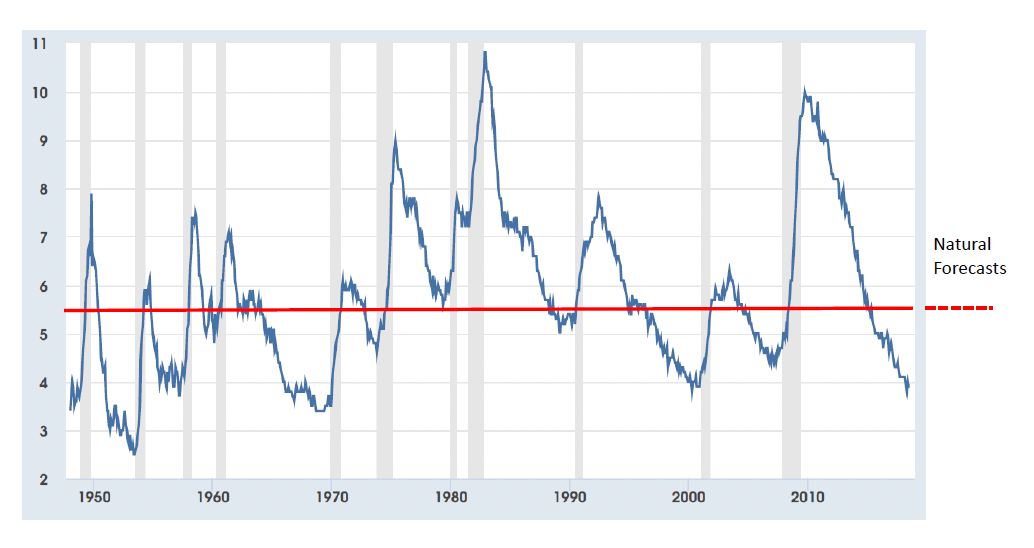
\includegraphics[width=\linewidth]{Capture d’écran 2025-10-14 à 22.10.43.png}
\end{figure}
\end{frame}



% ——————————————————————————————————————————
% Historical perspective: stationarity and linearity
% ——————————————————————————————————————————
\begin{frame}{Historical perspective on stationarity and linearity}
\small
\begin{itemize}
  \item Up to the end of the 1970s, time-series analysis assumed a \textbf{stationary and linear} setup.
  \item \textbf{Nelson and Plosser (JME, 1982):} applied \textbf{Dickey-Fuller tests} and showed that most \textbf{macroeconomic and financial time series are non-stationary}  
  $\Rightarrow$ statistical inference based on stationarity was \textbf{invalid}.
  \item More recently: \textbf{linearity tests} and new classes of models emerged:
  \begin{itemize}
    \item structural change and threshold models,
    \item stochastic volatility models.
  \end{itemize}
  \item \textbf{Example:} prices, interest rates, and financial time series are \textbf{nonlinear}.
  \item \textbf{Remark:} the non-stationarity issue is now acknowledged - but \textbf{still often within a linear, univariate framework (We will study nonlinear models!)}
\end{itemize}
\end{frame}

\begin{frame}{Summary}
\small
\begin{itemize}
  \item A TS is one observed realization of a stochastic process, thus its dependence structure requires assumptions on stability.
  \item \textbf{Stationarity} (constant mean, variance, covariance) is necessary for estimation, inference, and forecasting.
  \item Nonstationarity may stem from \textbf{deterministic trends}, \textbf{stochastic trends (unit roots)}, \textbf{seasonality}, \textbf{structural breaks}.
  \item To achieve stationarity:
    \begin{itemize}
        \item Log $\Rightarrow$ stabilize variance.
        \item Check ACF visually and test for unit roots:
        \begin{itemize}
            \item Detrend $\Rightarrow$ remove deterministic trend.
        \end{itemize}
        \begin{itemize}
            \item Or difference $\Rightarrow$ remove stochastic trend.
        \end{itemize}  
        \begin{itemize}
            \item Or filter $\Rightarrow$ separate frequency components (trend vs cycle).
        \end{itemize}
    \end{itemize}
  \item But: filtering is never neutral - it defines what counts as “trend” and “cycle.”  Misuse can distort macro interpretation.
  \item Once stationary: by \textbf{Wold’s theorem}, any process can be represented  as a linear combination of past shocks $\Rightarrow$ foundation for \textbf{AR, MA, ARMA models.}
\end{itemize}
\end{frame}





\end{document}

